\documentclass[11pt]{article}
\usepackage{graphicx,url,caption}
\usepackage{peder-macros}

\headsep 0.15in
\topmargin -.95in
\headheight 0.55in
\textheight 9in
\textwidth 7.0in
\oddsidemargin -0.4in
\evensidemargin -0.4in
\parindent 0in

\title{Math Concepts}
\author{Peder Larson, BI201 Fall 2011}
\begin{document}
\maketitle 

\section*{Complex Numbers}

$$c = a + i b = A\exp(i \phi)$$
$$ i = \sqrt{-1}, \,
\exp(i \phi) = \cos \phi + i \sin\phi$$
$$ |c| = A = \sqrt{a^2+b^2}$$
$$ \phi = \tan^{-1} (b/a)$$

\section*{Impulse Function}

The impulse (or delta) funcion, $\delta(x)$, can be used to represent sampling of a continuous signal, and has the following properties:
\begin{enumerate}
\item $\delta(x) = 0$ for all $x \ne 0$
\item $\delta(x) \rightarrow \infty$ at $x =0$
\item $\int_{-\infty}^\infty \delta(x) dx = 1$
\item $\delta(ax) = \frac{1}{|a|} \delta(x)$
\item $f(x) \delta(x) = f(0) \delta(x)$
\item $f(x) \ast \delta(x) = f(x)$
\end{enumerate}

\section*{Other Functions}
Rectangle function
$$\rect(x) = \sqcap(x) = 
\left\{ 
  \begin{array}{l l}
    1 & \quad |x| < 1/2 \\
    1/2 & \quad |x| = 1/2 \\
    0 & \quad |x| > 1/2 \\
  \end{array} \right. $$
\begin{center}
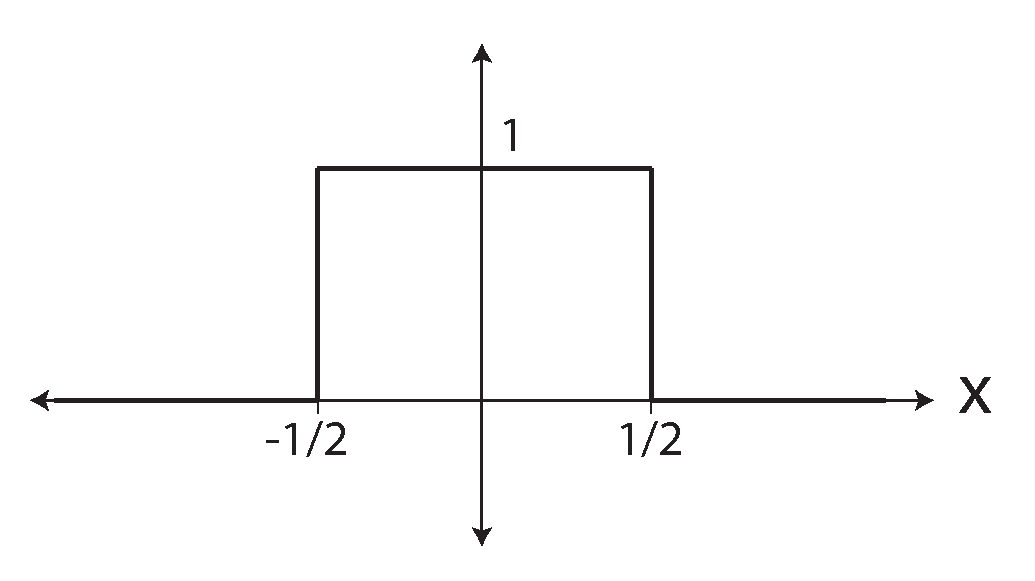
\includegraphics[width=.4\columnwidth]{rect.pdf}
\end{center}

Sinc
$$\sinc(x) = \frac{\sin(\pi x)}{\pi x}$$
\begin{center}
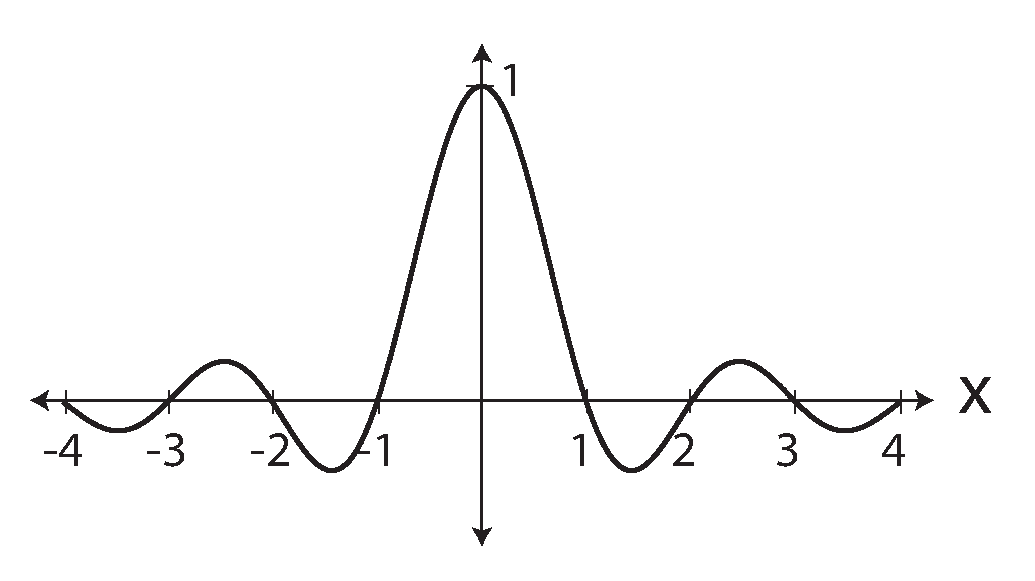
\includegraphics[width=.4\columnwidth]{sinc.pdf}
\end{center}

Comb/Shah (Impulse Train)
$$\Sha(x) = \sum_{n = -\infty}^\infty \delta(x - n)$$

\section*{Convolution}
The convolution operation $\ast$, is defined as:
$$ g(x) \ast h(x) = \int_{-\infty}^\infty g(x-\tau) h(\tau) d\tau$$

\section*{Fourier Transforms}

The Fourier transform, $ \mathcal{F} \{ \cdot \}$ of a complex-valued function, $f(x)$ is:
$$ \mathcal{F} \{ f(x) \} = F(k_x) = \int_{-\infty}^\infty f(x) \exp(-i 2 \pi k_x x) dx$$

Inverse Fourier Transform:
$$ \mathcal{F}^{-1} \{ F(k_x) \} = f(x) = \int_{-\infty}^\infty F(k_x) \exp(+i 2 \pi x k_x) dk_x$$

2-D Fourier Transform
$$ F(k_x,k_y) = \int_{-\infty}^\infty \int_{-\infty}^\infty f(x,y) \exp(-i 2 \pi (k_x x + k_y y) ) dx dy$$

N-D Fourier Transform
$$ F(\vec{k}) = \int_{-\infty}^\infty f(\vec{x}) \exp(-i 2 \pi \vec{k}\cdot \vec{x}) d\vec{x}$$

Duality
$$\mathcal{F}\{f(x)\} = F(k_x)$$
$$\mathcal{F}\{F(x)\} = f(-k_x)$$
$$\mathcal{F}\{F(-x)\} = f(k_x)$$

Separable

If $f(x,y) = f_x(x) f_y(y)$, then $\mathcal{F}\{f(x,y)\} = \mathcal{F}\{f_x(x)\} \mathcal{F}\{f_y(y)\}$


\subsection*{Transform Identities and pairs}
For 
$\mathcal{F}\{f(x)\} = F(k_x), \mathcal{F}\{g(x)\} = G(k_x)$:
\begin{center}
\begin{tabular}{|c|c|}
\hline
Function & Fourier Transform\\
\hline
$\delta(x)$ & 1 \\
1 & $\delta(k_x)$ \\
$\mathrm{rect}(x)$ & $\mathrm{sinc}(k_x)$ \\
$f(ax)$ & $\frac{1}{|a|} F(\frac{k_x}{a})$\\
$a \cdot f(x) + b \cdot g(x)$ & $a \cdot F(k_x) + b \cdot G(k_x)$ \\
$f(x-a)$ & $\exp(-i 2\pi a k_x) F(k_x)$\\
$\exp(i 2\pi a x) f(x)$ & $F(k_x - a)$\\
$f(x) \ast g(x)$ & $F(k_x) G(k_x)$ \\
$f(x) g(x)$ & $F(k_x) \ast G(k_x)$ \\
\hline
\end{tabular}
\end{center}

\end{document}